Our preliminary evaluation demonstrates that this approach shows a lot of
promise. However, investigation into better replacement policies will
likely yield improvements in system performance.

\subsection{Methodology}

In our experimental setup, we generated key-value pairs, placed them in
memcached, and performed a GET request for each key. We then measured the
latencies for a series of GET requests generated from a predetermined
probability distribution. These distributions include one checking only a
single key, a uniform distribution, a normal distribution, a Pareto
distribution, and a distribution based on the ETC workload from a Facebook
study \cite{AXFJP2012}.

\subsection{Results}

In our first benchmark, we compared the latency of our accelerator to the
latency of software memcached in responding to requests for a single key.
For this experiment, we set a single key on the accelerator and in the
unmodified memcached software. We then issued repeated GET requests with
small random delays in between and recorded the latency of each request.

\begin{figure}[t]
\begin{center}
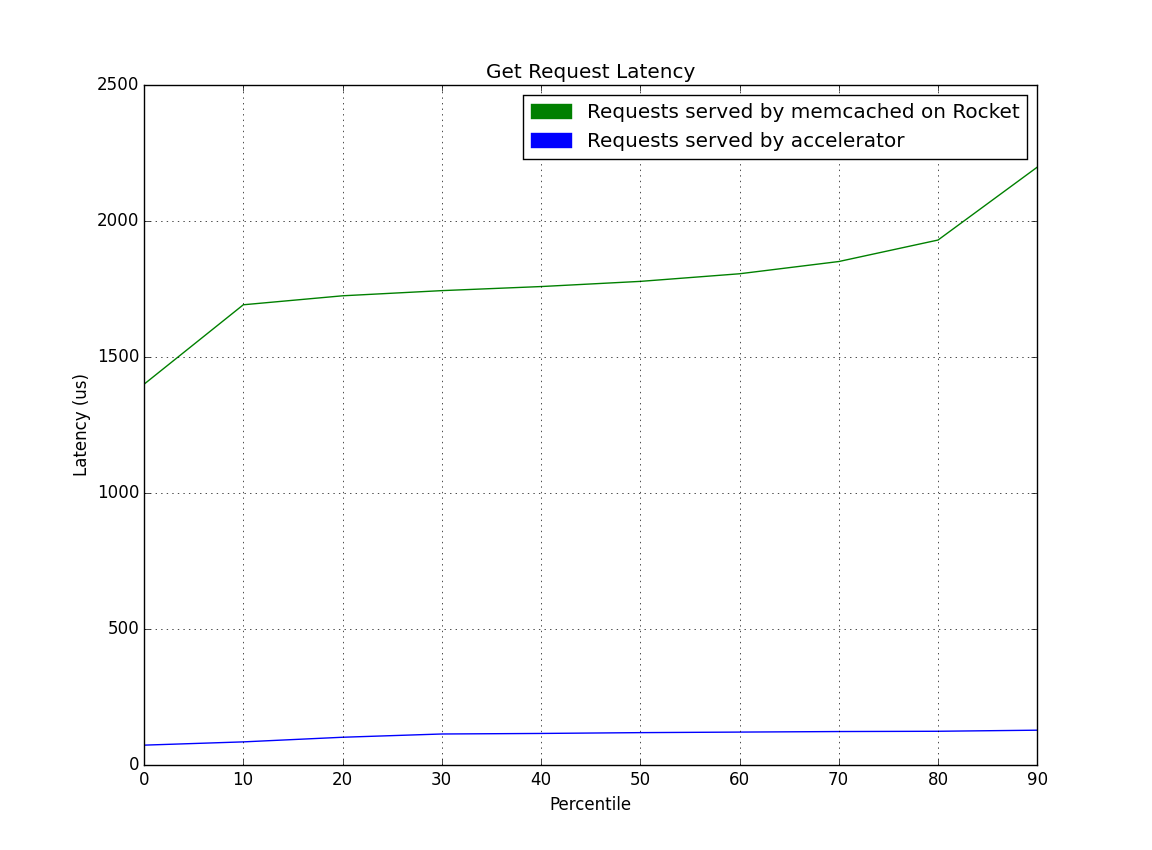
\includegraphics[width=\linewidth]{graph.png}
\caption{Latency of GET requests when only getting 1 key}
\label{fig:one-req}
\end{center}
\end{figure}

\begin{figure}[t]
\begin{center}
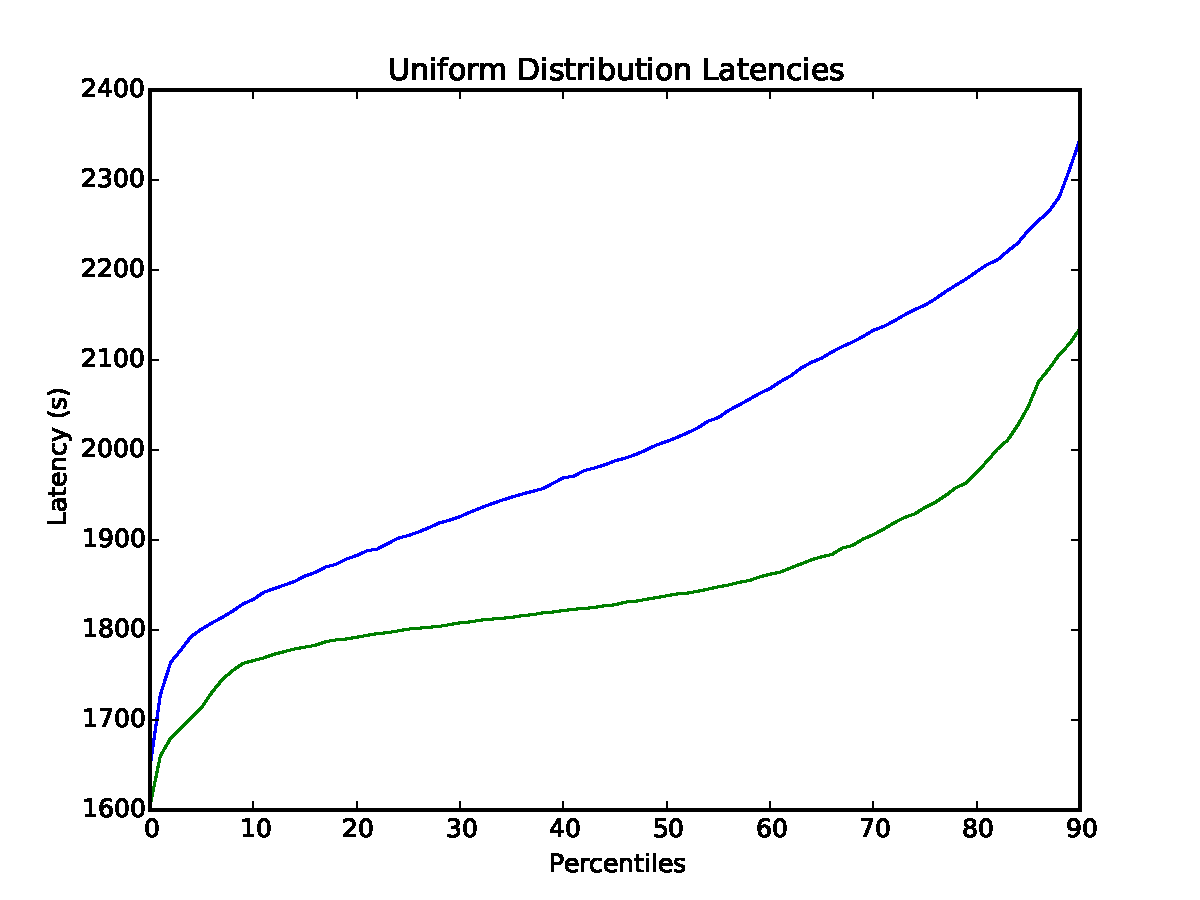
\includegraphics[width=\linewidth]{unif.pdf}
\caption{Latency of GET requests when keys follow a uniform distribution}
\label{fig:unif}
\end{center}
\end{figure}

\begin{figure}[t]
\begin{center}
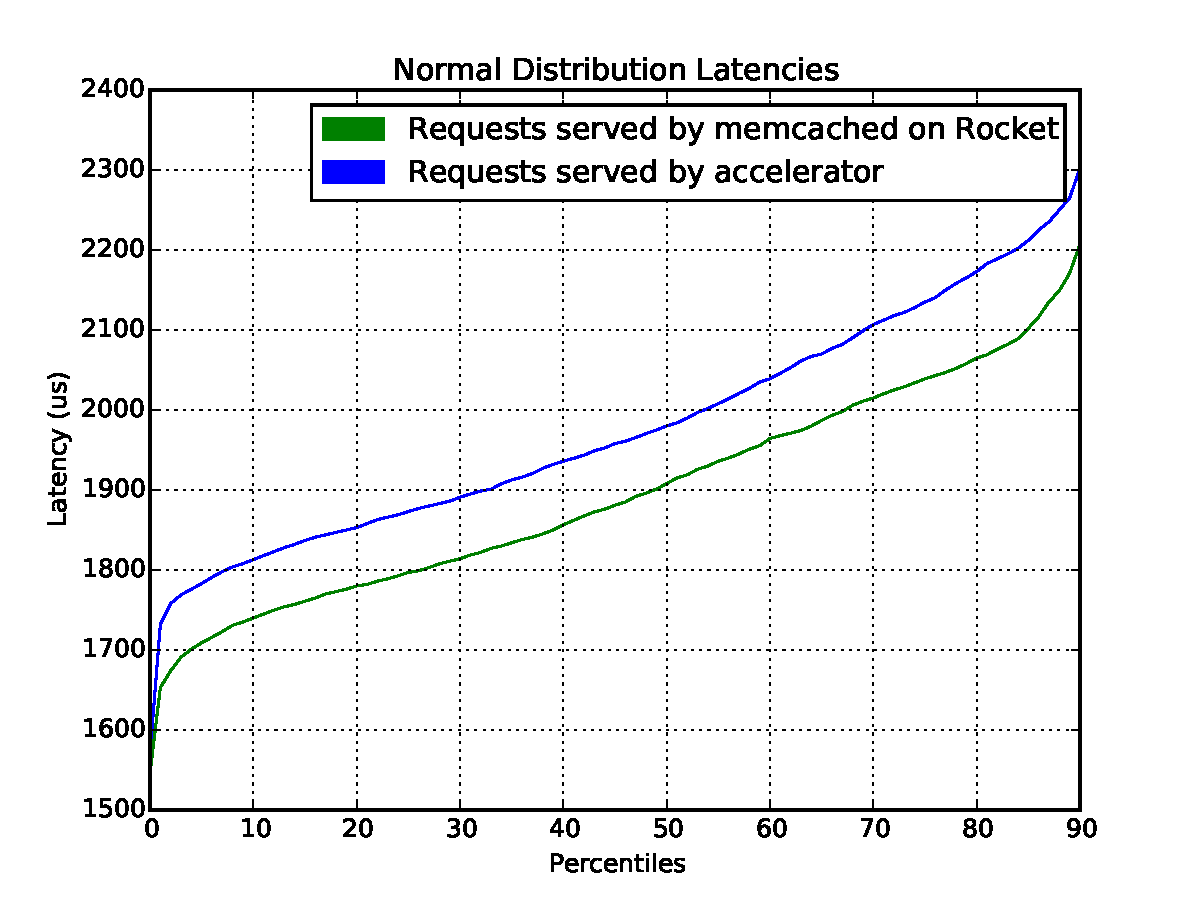
\includegraphics[width=\linewidth]{norm.pdf}
\caption{Latency of GET requests when keys follow a normal distribution}
\label{fig:norm}
\end{center}
\end{figure}

As we see from Figure \ref{fig:one-req}, there is approximately an order of
magnitude improvement between a request served by the accelerator and a
request served by memcached software running on the CPU.

After the single-key benchmark, we tested a series of requests chosen
according to a uniform distribution of keys.

In Figure \ref{fig:unif}, we see that, for this distribution, the
hardware-accelerated implementation performs worse than than the pure software
implementation. The driving factor behind the poor performance is the overhead
incurred in the traffic manager when checking whether each key is in the accelerator.
Since all requests on the accelerated implementation must pay this penalty,
we expect the accelerated implementation to perform poorly for key
distributions that are not heavily skewed. The results for a normal distribution
(Figure \ref{fig:norm}) show similarly poor performance for the accelerator
compared to the software implementation.

\begin{figure}[t]
\begin{center}
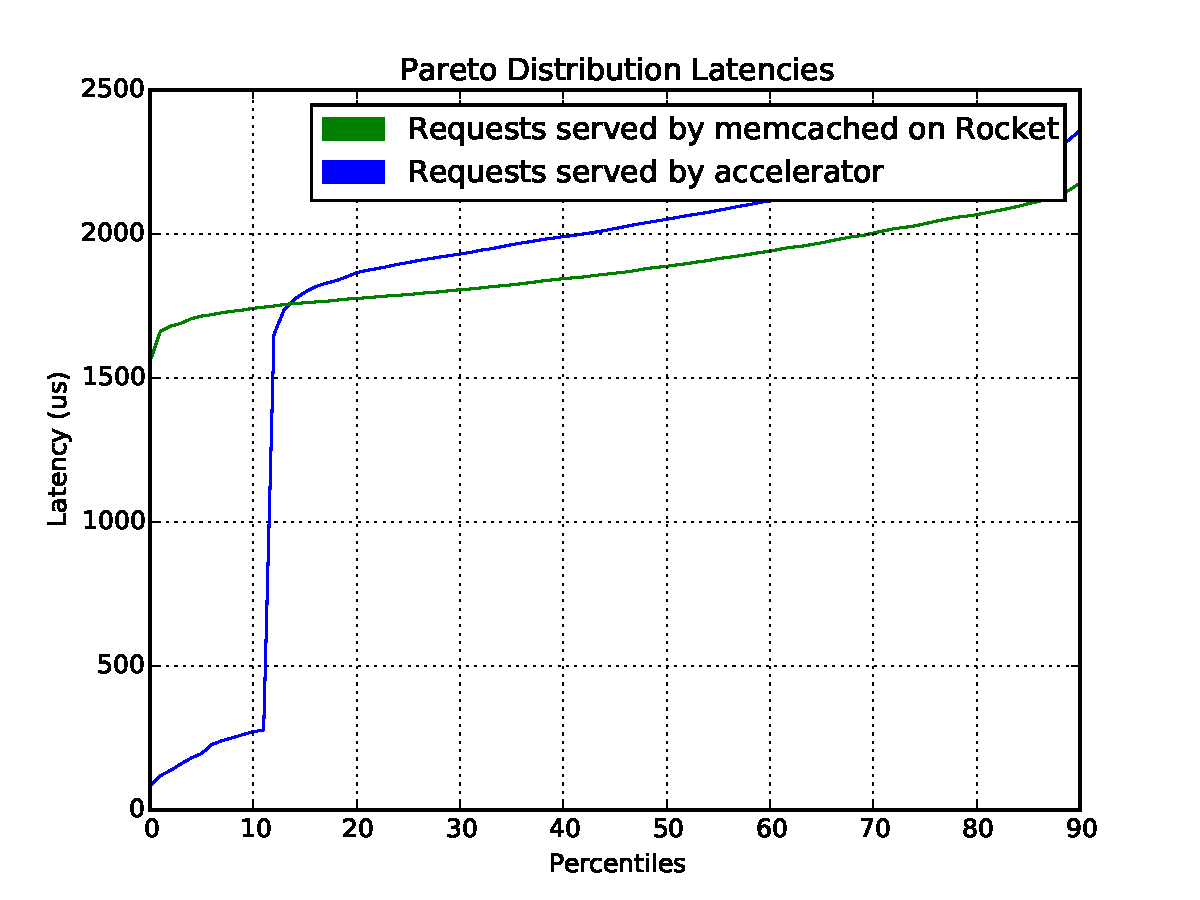
\includegraphics[width=\linewidth]{pareto.pdf}
\caption{Latency of GET requests when keys follow a pareto distribution}
\label{fig:pareto}
\end{center}
\end{figure}

\begin{figure}[t]
\begin{center}
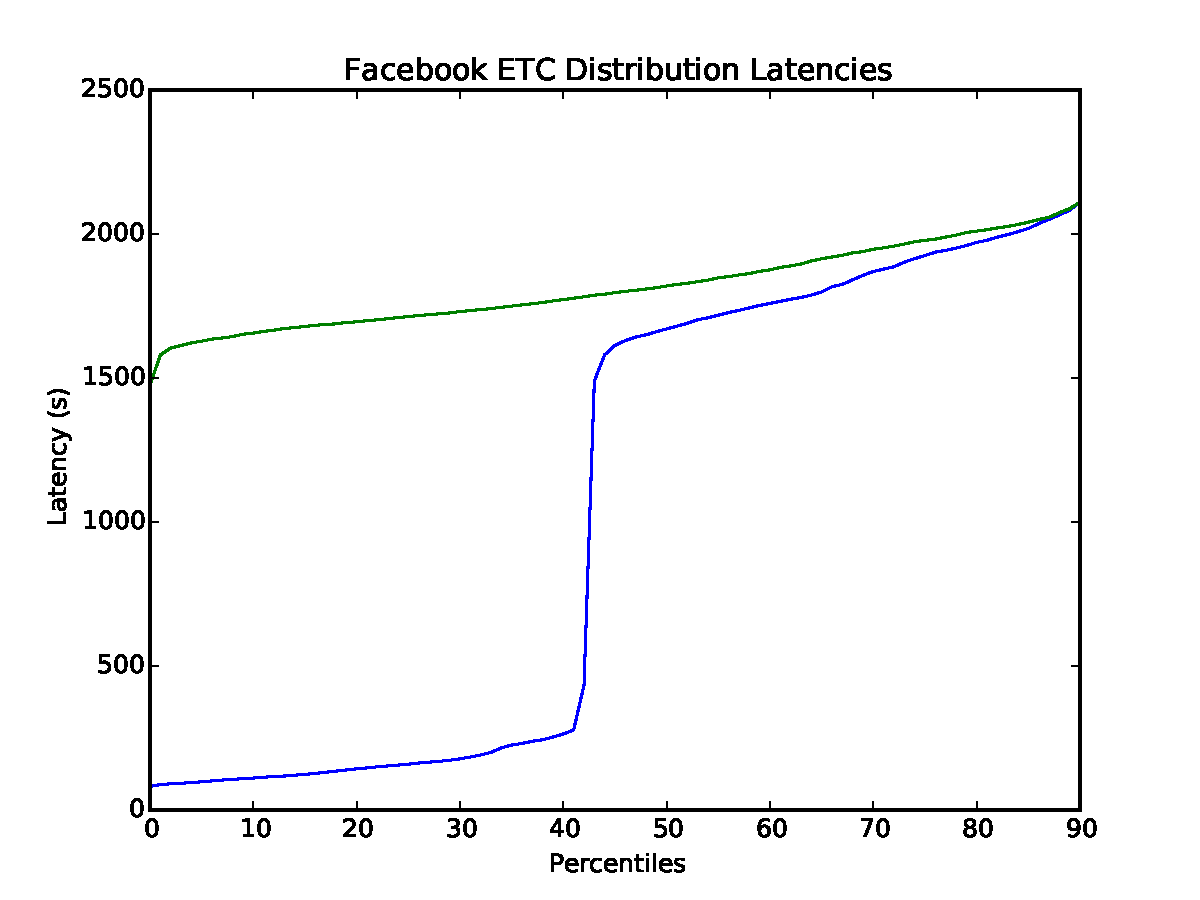
\includegraphics[width=\linewidth]{etc.pdf}
\caption{Latency of GET requests when keys follow the Facebook ETC distribution}
\label{fig:etc}
\end{center}
\end{figure}

For skewed distributions such as a Pareto distribution (Figure \ref{fig:pareto}),
we see a drastic improvement in the accelerated implementation over the
pure-software implementation. In this test, the most popular keys are placed
on the accelerator and are not easily evicted. For the these keys, the 10x
latency improvement from serving from the accelerator more than makes up
for the latency penalty incurred in the traffic manager. However, only about
$11\%$ of the requests benefit from acceleration. Requests for keys not placed
on the  accelerator still have higher latency than in the software implementation.

Finally, we used the Facebook ETC distribution \cite{AXFJP2012} in order to see
how our system would fare against a more realistic workload. In Figure
\ref{fig:etc}, we see that this is a very promising start. $40$ percent of all
requests get a factor-of-ten improvement in latency. However, the poor
performance in the non-skewed distributions suggests that improvements can be
made in our caching policy to enhance system performance.
